% \documentclass{book}

\documentclass[12pt]{article}
\usepackage[pdfborder={0 0 0.5 [3 2]}]{hyperref}%
\usepackage[left=1in,right=1in,top=1in,bottom=1in]{geometry}%
\usepackage[shortalphabetic]{amsrefs}%
\usepackage{amsmath}
\usepackage{enumerate}
\usepackage{enumitem}
\usepackage{amssymb}                
\usepackage{amsmath}                
\usepackage{amsfonts}
\usepackage{amsthm}
\usepackage{bbm}
\usepackage[table,xcdraw]{xcolor}
\usepackage{tikz}
\usepackage{float}
\usepackage{booktabs}
\usepackage{svg}
\usepackage{mathtools}
\usepackage{cool}
\usepackage{url}
\usepackage{graphicx,epsfig}
\usepackage{makecell}
\usepackage{array}

\def\noi{\noindent}
\def\T{{\mathbb T}}
\def\R{{\mathbb R}}
\def\N{{\mathbb N}}
\def\C{{\mathbb C}}
\def\Z{{\mathbb Z}}
\def\P{{\mathbb P}}
\def\E{{\mathbb E}}
\def\Q{\mathbb{Q}}
\def\ind{{\mathbb I}}

\graphicspath{ {images/} }

\begin{document}

\section{Introduction}

\section{Numerics}

\subsection{Parameter Continuation}

\subsection{Double Pulse Construction}

\begin{figure}[H]
	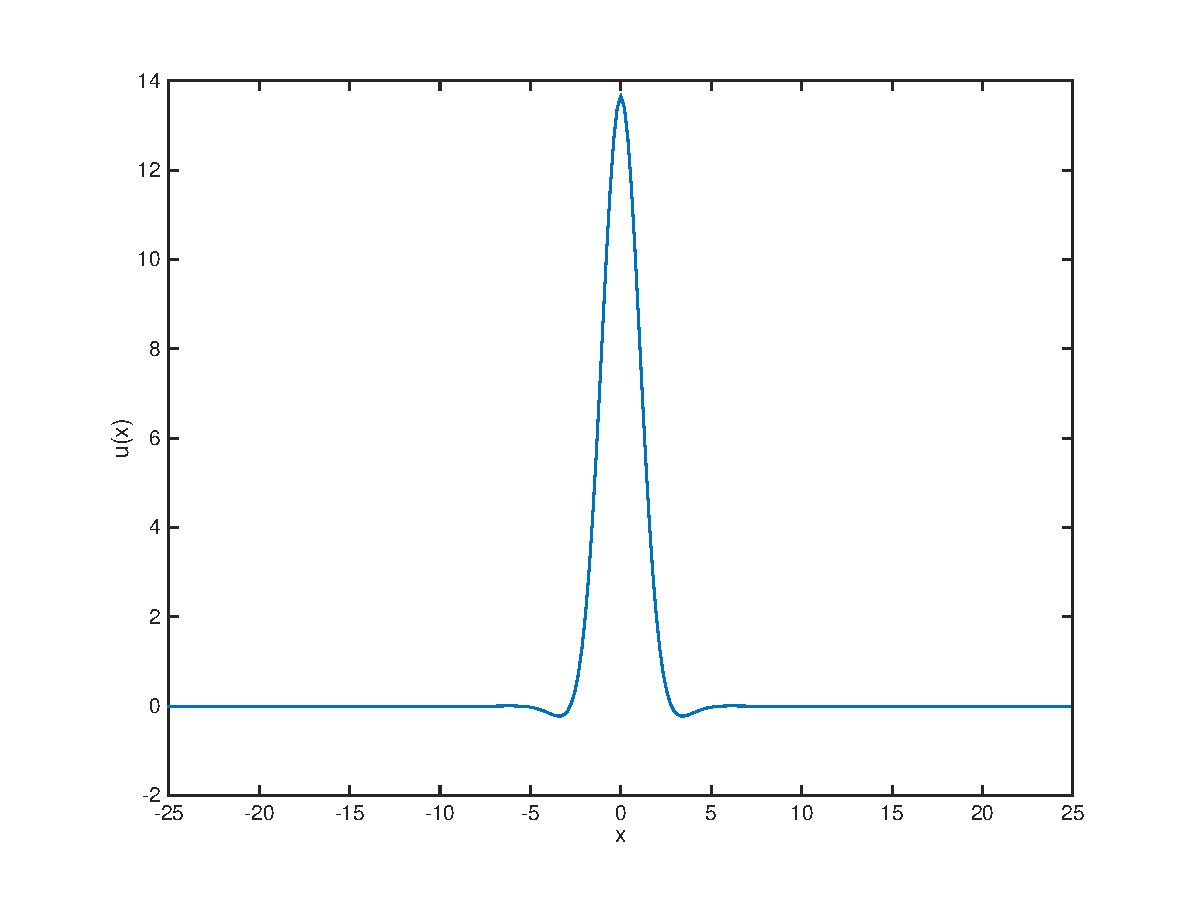
\includegraphics[width=8.5cm]{four10primary.eps}
	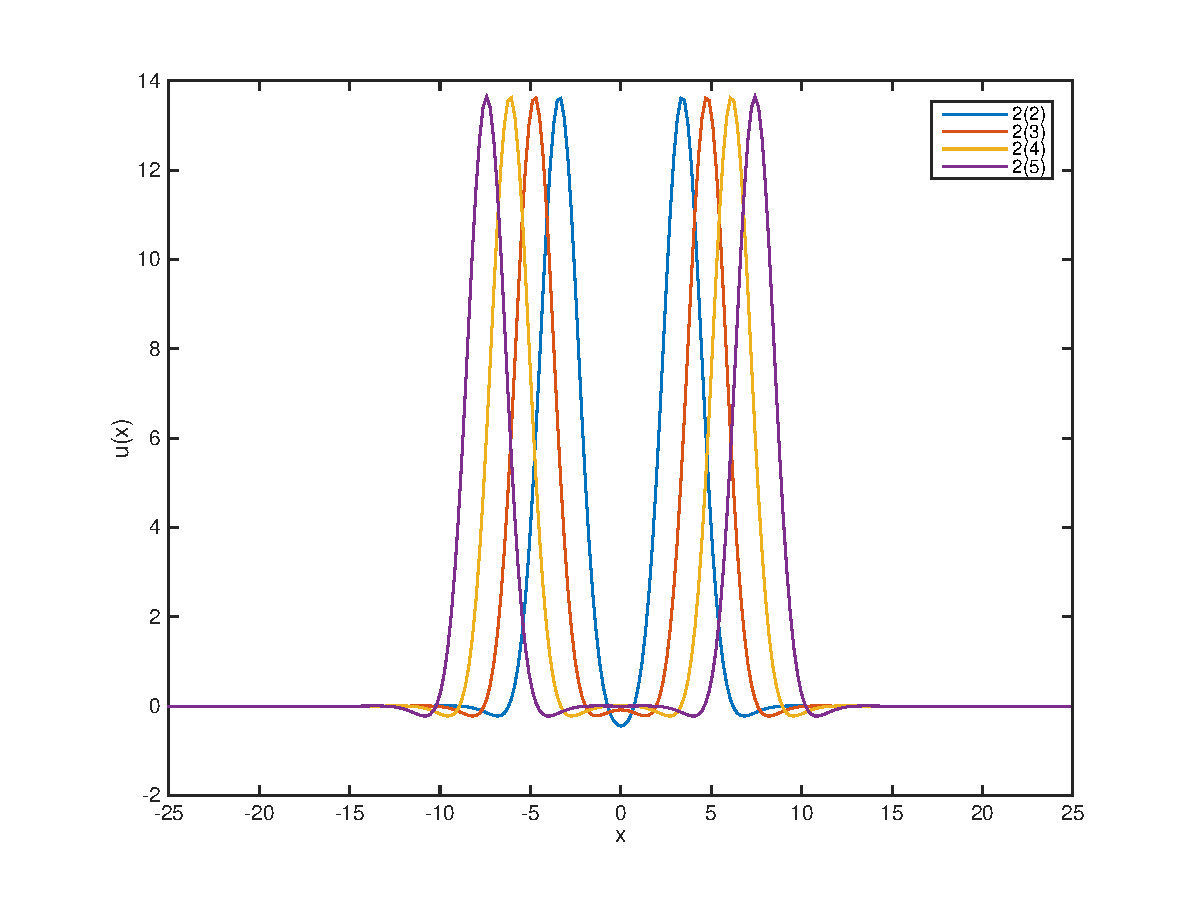
\includegraphics[width=8.5cm]{four10double.eps}
	\caption{Primary pulse and double pulses 2(2), 2(3), 2(4), and 2(5). Fourier spectral methods, $N = 256$, wave speed $c = 10$.}
\end{figure}

Roots of linearization about 0 solution are $\alpha + \beta i = \pm1.3532 \pm 1.1537i$.

\begin{figure}[H]
	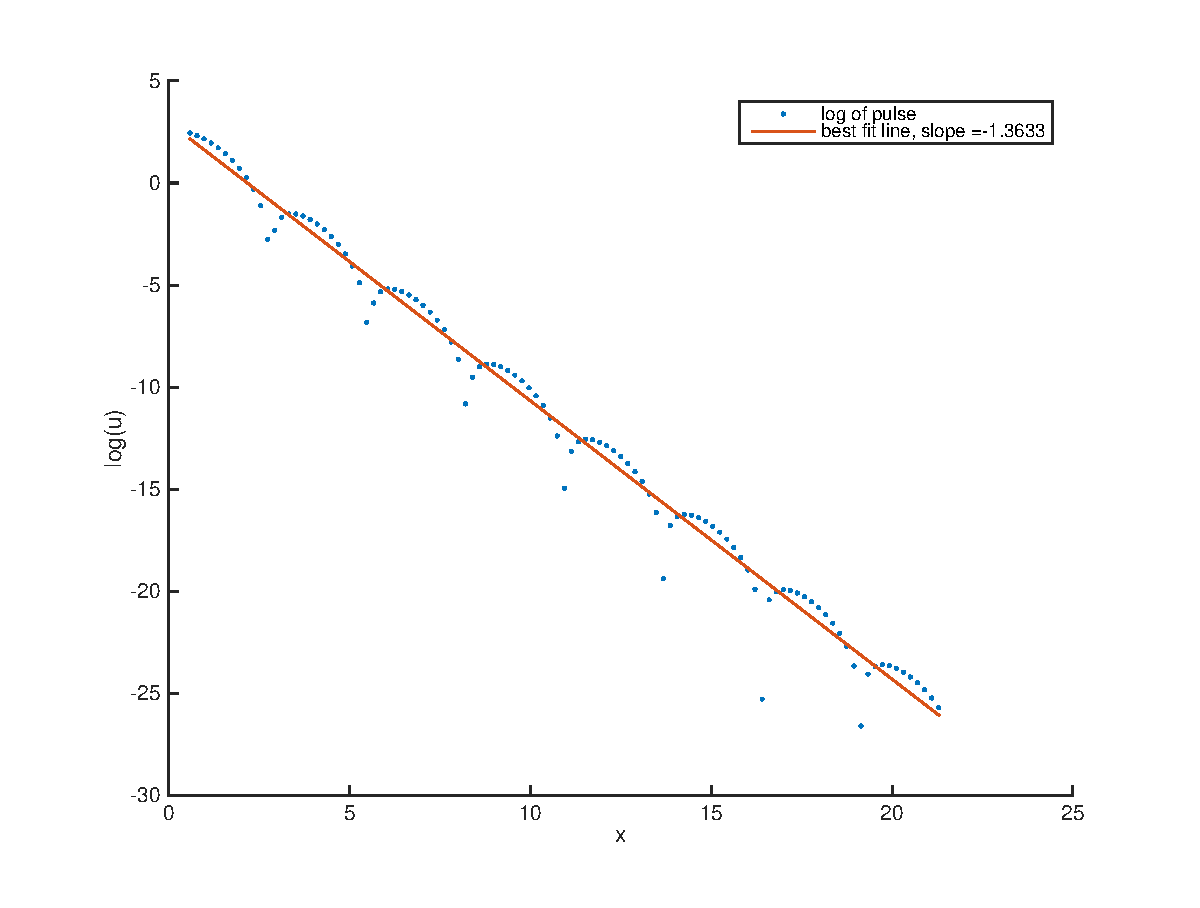
\includegraphics[width=8.5cm]{decaysinglepulse.eps}
	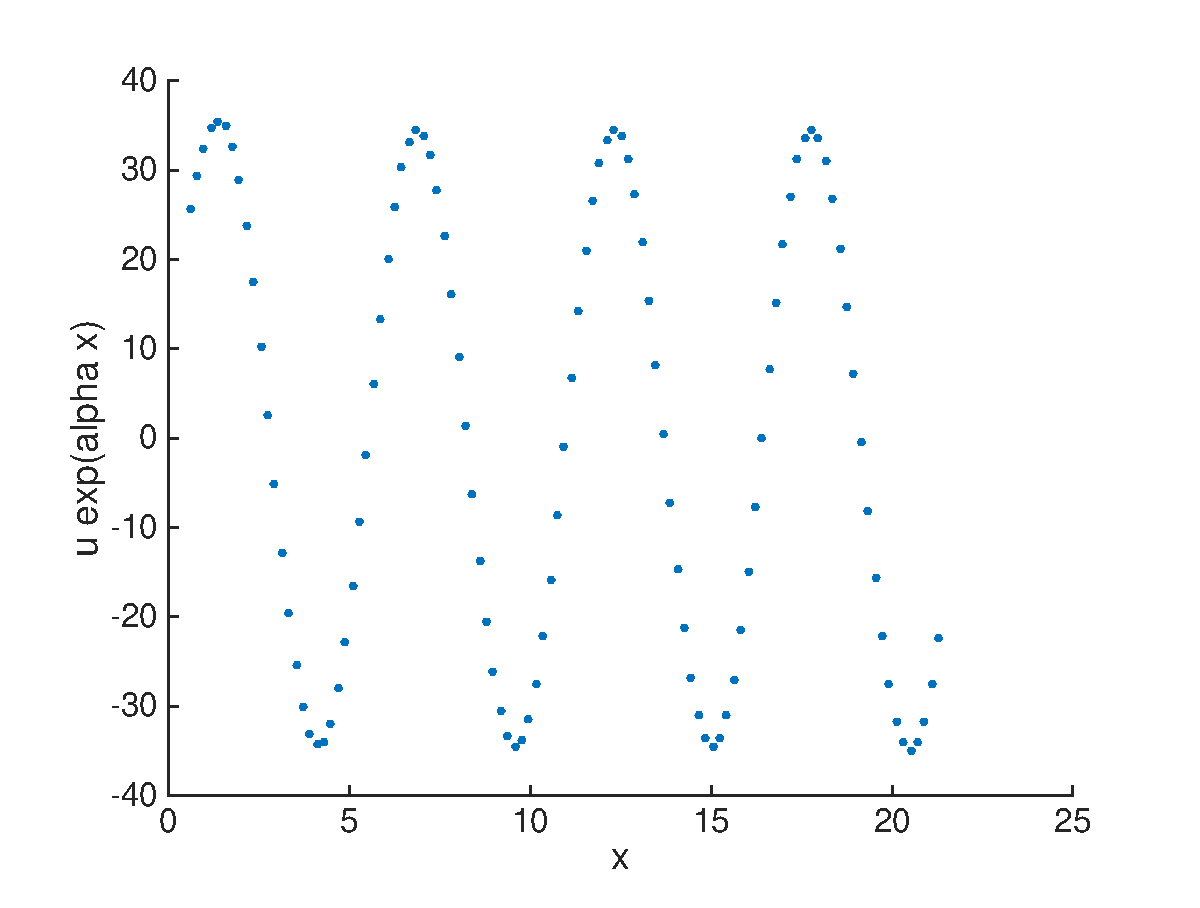
\includegraphics[width=8.5cm]{oscsinglepulse.eps}
	\caption{For single pulse $u(x)$, plot of $\log u(x)$ (left) and $e^{\alpha x} u(x)$ (right). Slope of best fit line on left is -1.3633, which is approximately $\alpha$. Period on right is 5.4688, frequency is 1.1489, which is approximately $\beta$.}
\end{figure}

\begin{figure}[H]
	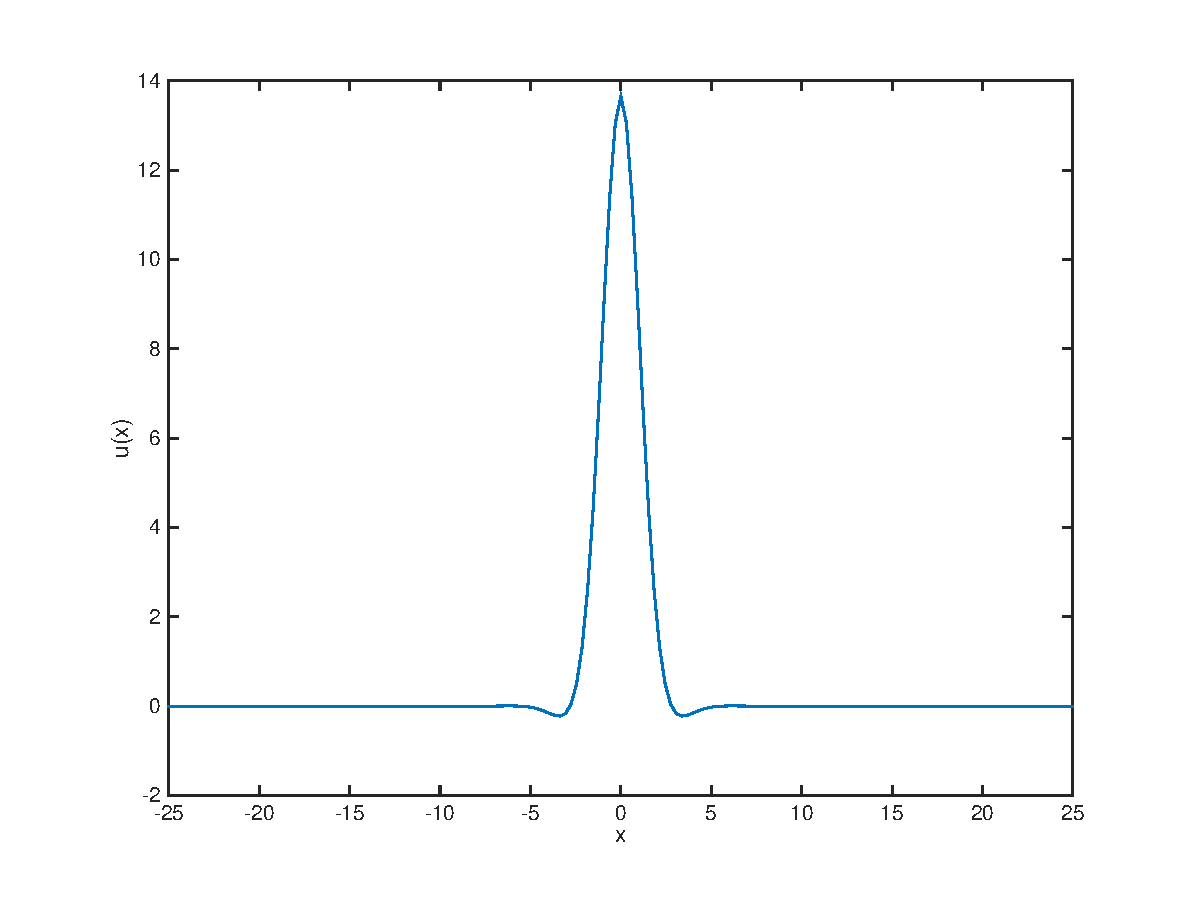
\includegraphics[width=8.5cm]{cheb10primary.eps}
	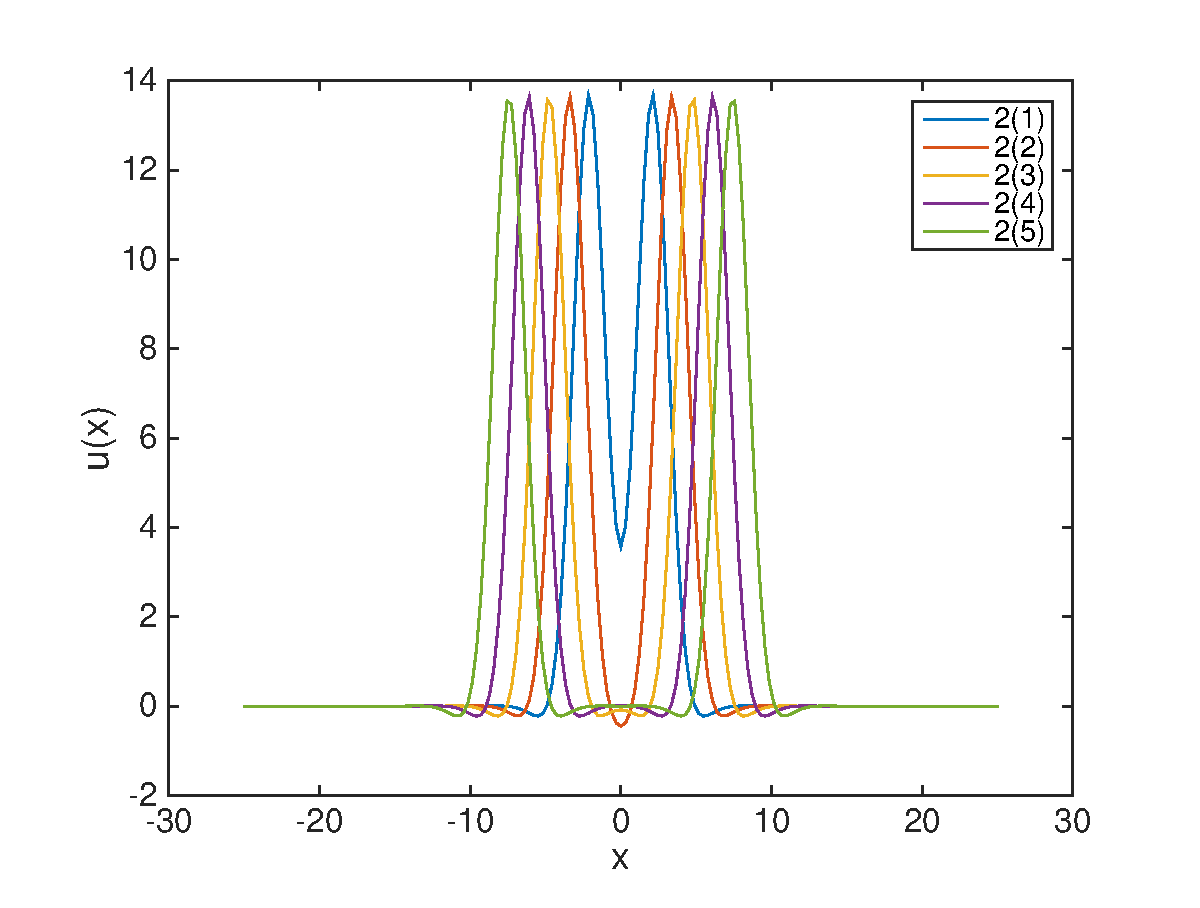
\includegraphics[width=8.5cm]{cheb10double}
		\caption{Primary pulse and double pulses 2(2), 2(3), 2(4), and 2(5). Chebyshev spectral methods, $N = 257$, wave speed $c = 10$. }
\end{figure}

\subsection{Eigenvalues and Eigenfunctions}

(4th order eq) For double pulses, we should have a pair near 0 and a pair of negative eigenvalues. This is indeed the case. The table below just shows these eigenvalues. As expected, the paired eigenvalue near switches sides each time, so this is also good.

\begin{figure}[H]
\begin{tabular}{l|ll|ll}
Pulse  & Eigenvalue near 0  & Paired eigenvalue & Negative eigenvalue & Paired eigenvalue \\ \hline
1      & -5.5437e-12        &                   & -11.4747            &                   \\
2(2)   & 3.6523e-12         & 0.0326            & -11.4720            & -11.4695          \\
2(3)   & -2.4674e-12        & -0.0008           & -11.4748            & -11.4748          \\
2(4)   & 2.3849e-12         & 2.0506e-05        & -11.4747            & -11.4747          \\
2(5)   & -2.4082e-12        & -7.1428e-07       & -11.4747            & -11.4747          \\
\end{tabular}
\caption{Eigenvalues of 4th order operator for linearization about single pulse 1 and double pulses 2(2), 2(3), 2(4), and 2(5) for wave speeds $c = 10, 7.5, 5$. Fourier spectral methods, $N = 256$}
\end{figure}


\begin{figure}[H]
\begin{tabular}{l|lll}
 Double Pulse   & $c = 10$            & $c=7.5$                         & $c=5$        \\ \hline
  2(2) &     $\pm 0.4352$             & $\pm 0.2730$                    & $\pm 0.1363$ \\ 
  2(3) &     2.0829e-11 $\pm 0.0691i$ & -2.7698e-11 $\pm 0.0413i$       & 2.6806e-11 $\pm 0.0190i$\\ 
  2(4) &     $\pm 0.0109$             & $\pm 0.0062$                    & \\ 
  2(5) &    -8.5834e-13 $\pm 0.0020i$ & 6.8791e-12 $\pm$ 8.8812e-04$i$  & \\
\end{tabular}
\caption{Nonzero eigenvalues of 5th order operator for linearization about double pulses 2(2), 2(3), 2(4), and 2(5) for wave speeds $c = 10, 7.5, 5$. Fourier spectral methods, $N = 256$}
\end{figure}

\begin{figure}[H]
	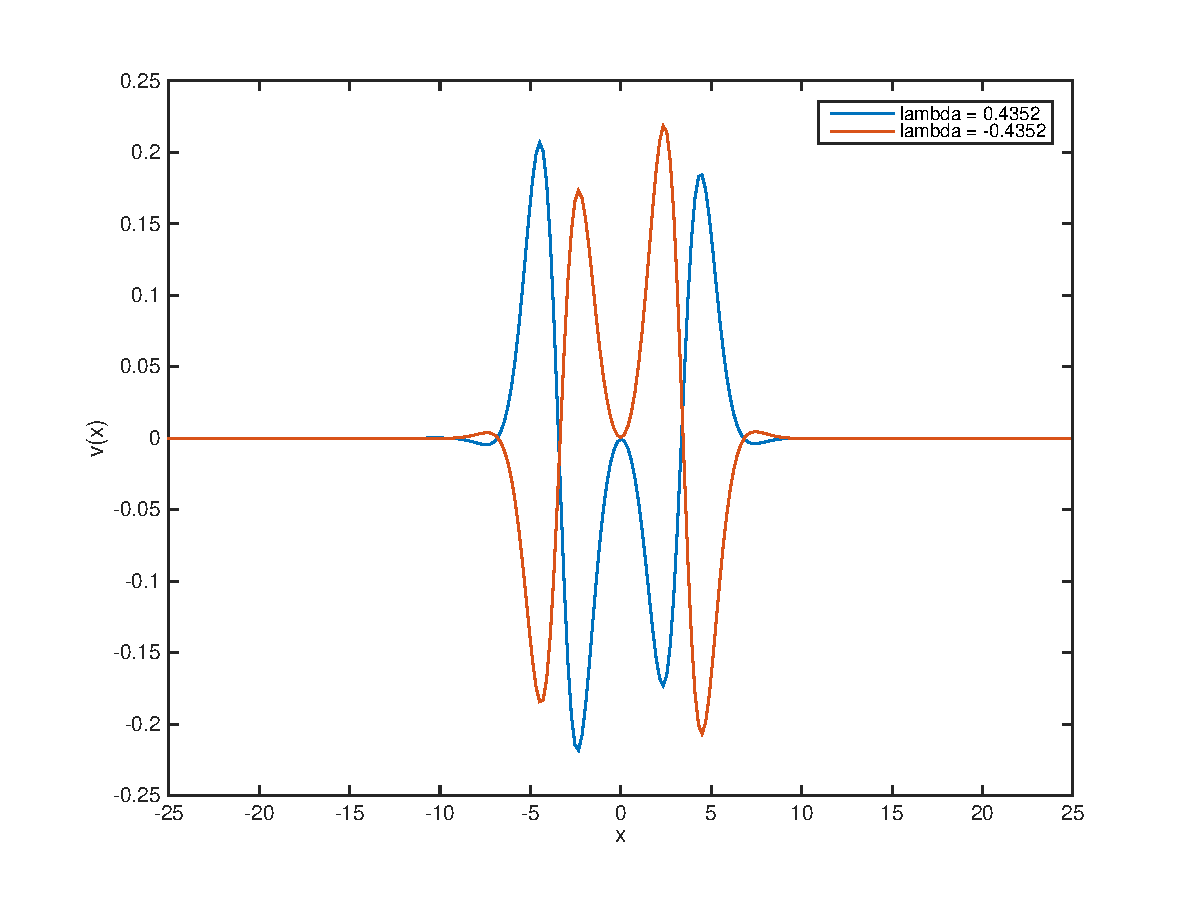
\includegraphics[width=8.5cm]{four10dp1eigenfns}
	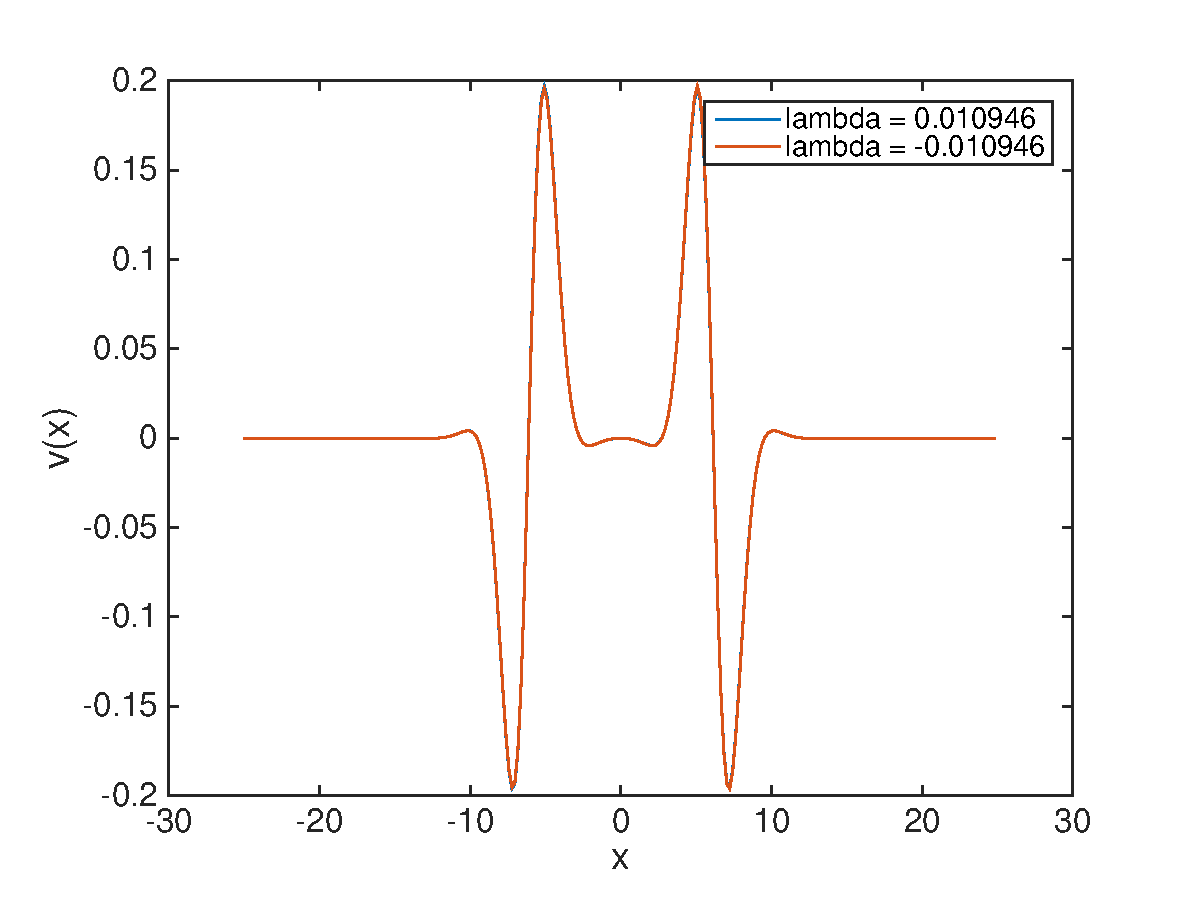
\includegraphics[width=8.5cm]{four10dp3eigenfns}
	\caption{Eigenfunctions corresponding to eigenvalues for linearization about double pulses 2(3) and 2(5) for wave speed $c = 10$, Fourier spectral methods, $N = 256$}
\end{figure}

For linearization about 0 solution, eigenvalue 0.4352, roots of characteristic polynomial are $-1.3639 \pm 1.1556i, 1.3422 \pm 1.1521i$.

\begin{figure}[H]
	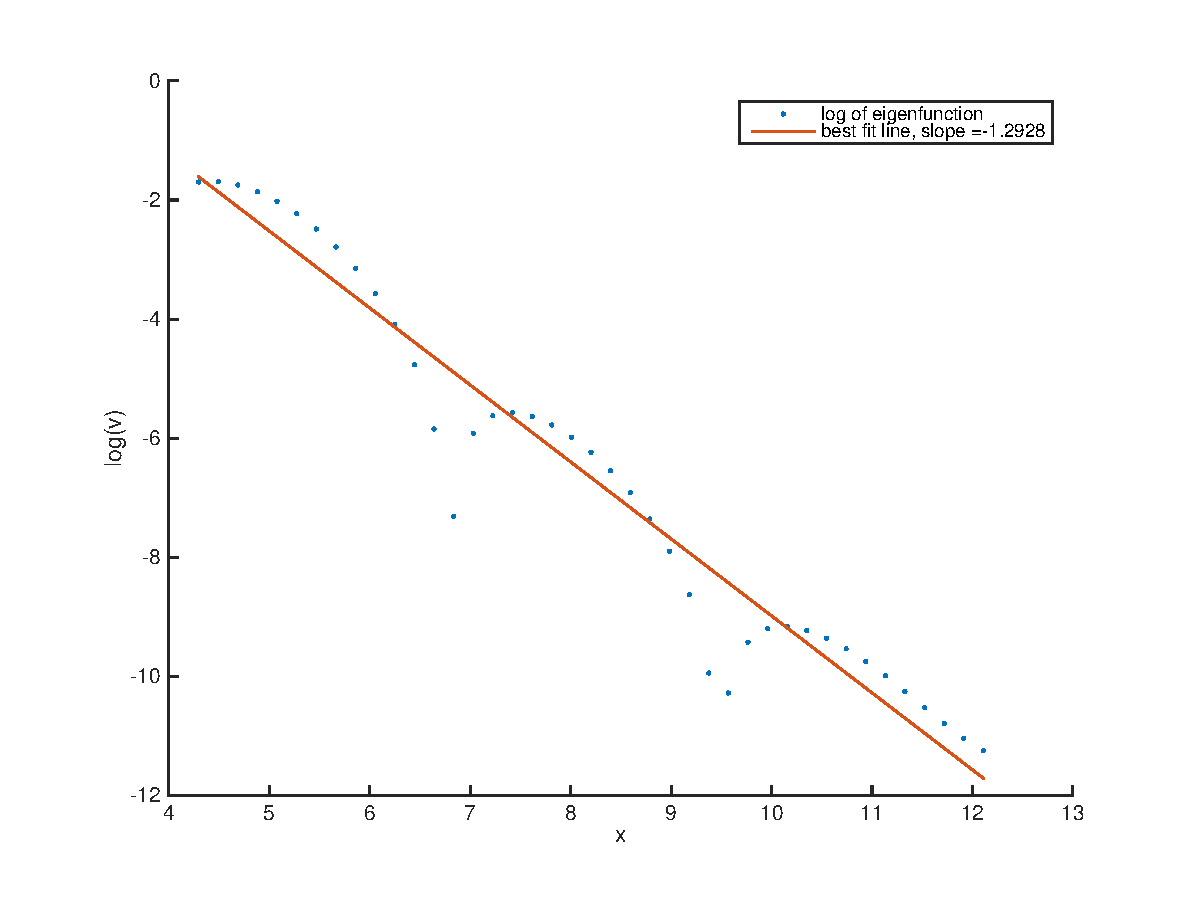
\includegraphics[width=8.5cm]{decayeigenfunction}
	\caption{For eigenfunction $v(x)$ corresponding to double pulse 2(2) with eigenvalues 0.4352, plot of $\log v(x)$. Slope of best fit line on left is -1.2928, which is close to the real parts of the roots above.}
\end{figure}

\begin{figure}[H]
	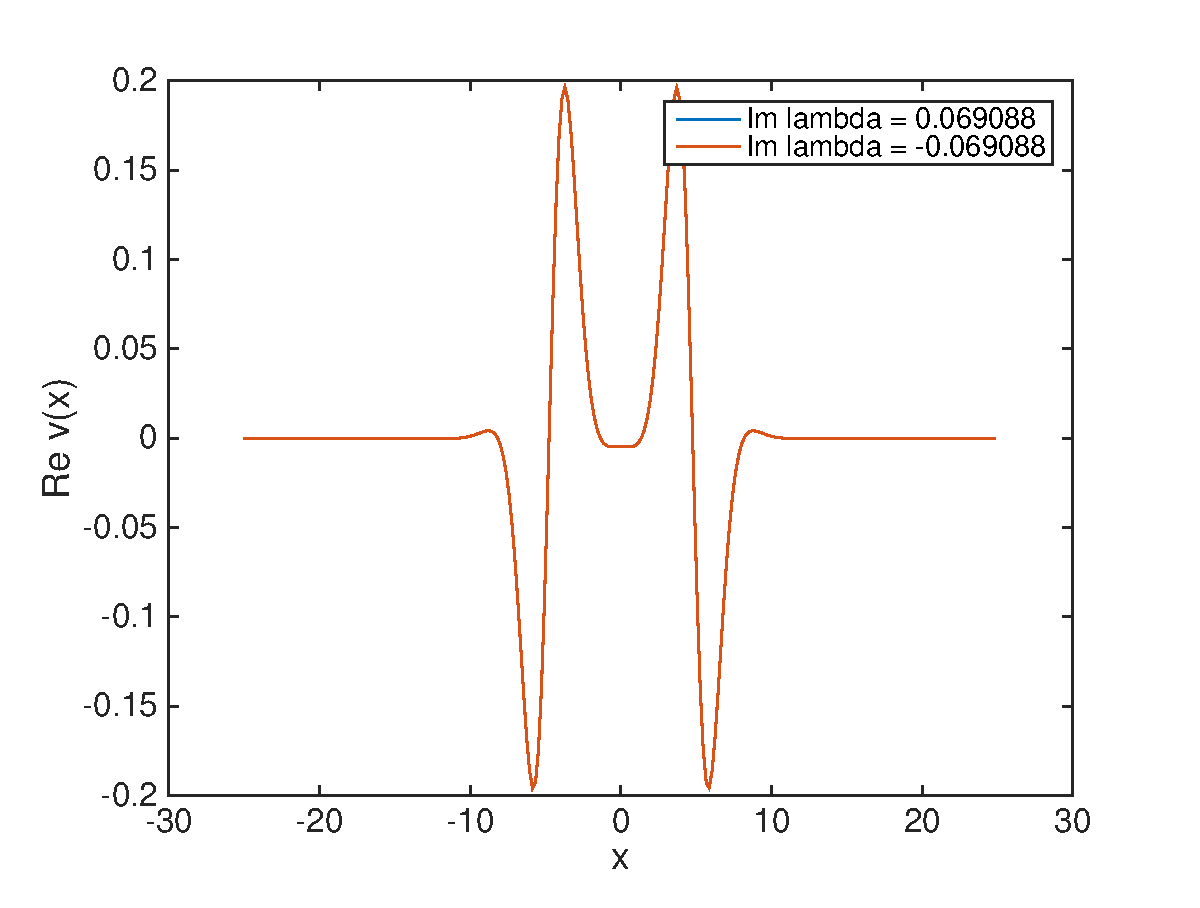
\includegraphics[width=8.5cm]{four10dp2eigenfnsreal}
	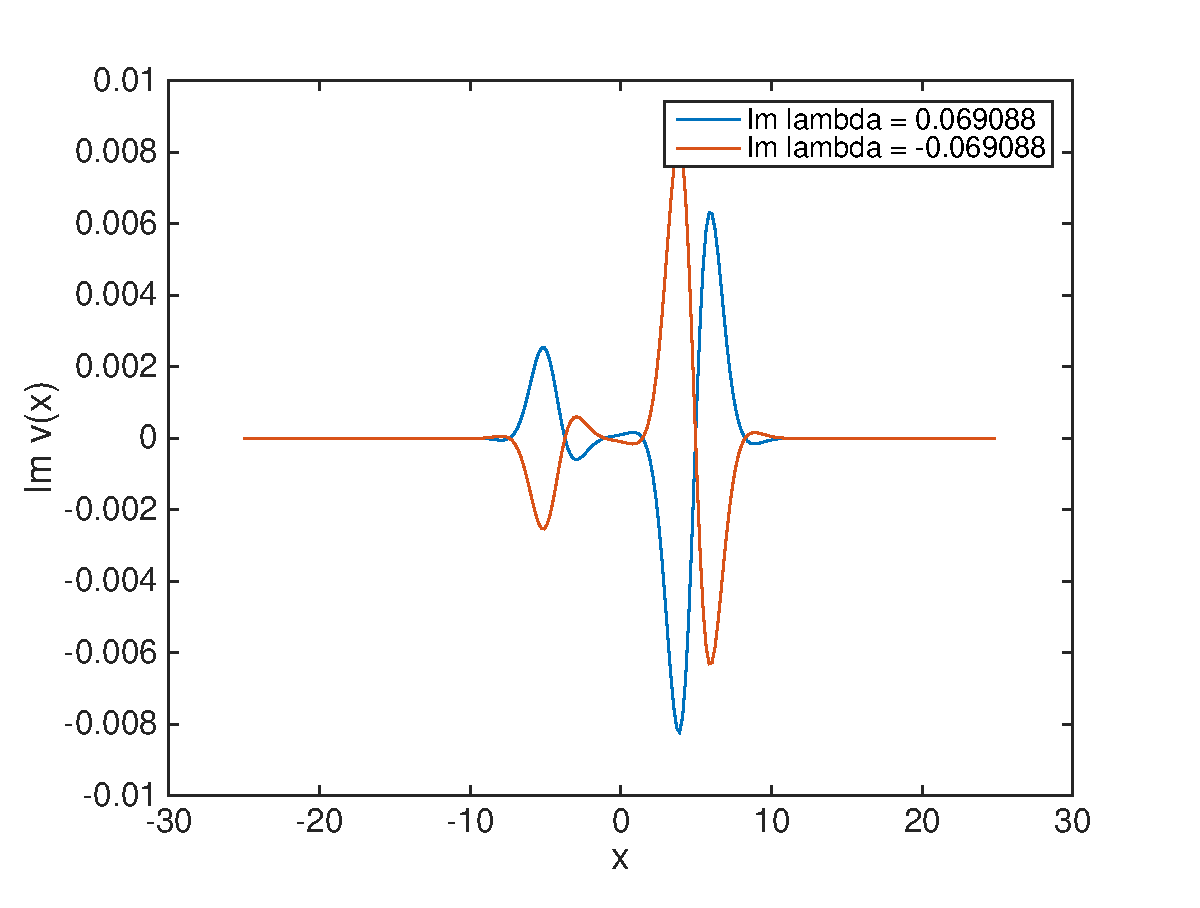
\includegraphics[width=8.5cm]{four10dp2eigenfnsimag}
	\caption{Real and imaginary parts of eigenfunctions corresponding to eigenvalues for linearization about double pulse 2(4) for wave speed $c = 10$, Fourier spectral methods, $N = 256$}
\end{figure}

\begin{figure}[H]
\begin{tabular}{l|ll}
 Double Pulse   & $\max{|Jv - \lambda v|}$ before \texttt{fsolve} & $\max{|Jv - \lambda v|}$ after \texttt{fsolve}\\ \hline
  2(3) & 4.4440e-11 & 7.2469e-12 \\
  2(5) & 5.3975e-11 & 5.5005e-12 \\
\end{tabular}
\caption{Maximum of eigenvalue problem $|Jv - \lambda v|$ before and after using Matlab's \texttt{fsolve} to eliminate small real part of eigenvalue. Wave speed $c = 10$, Fourier spectral methods, $N = 256$.}
\end{figure}

\begin{figure}[H]
	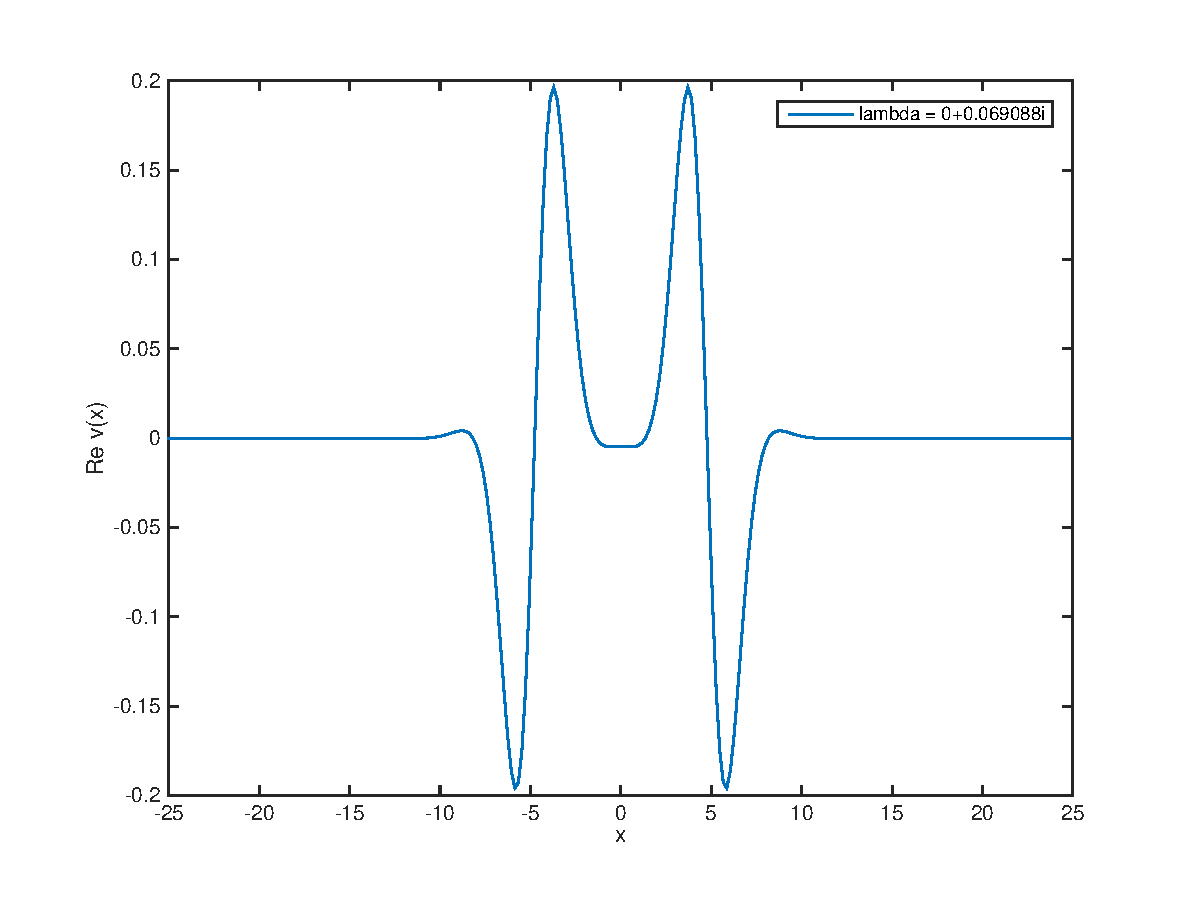
\includegraphics[width=8.5cm]{four10dp2eigenfnsreal_after}
	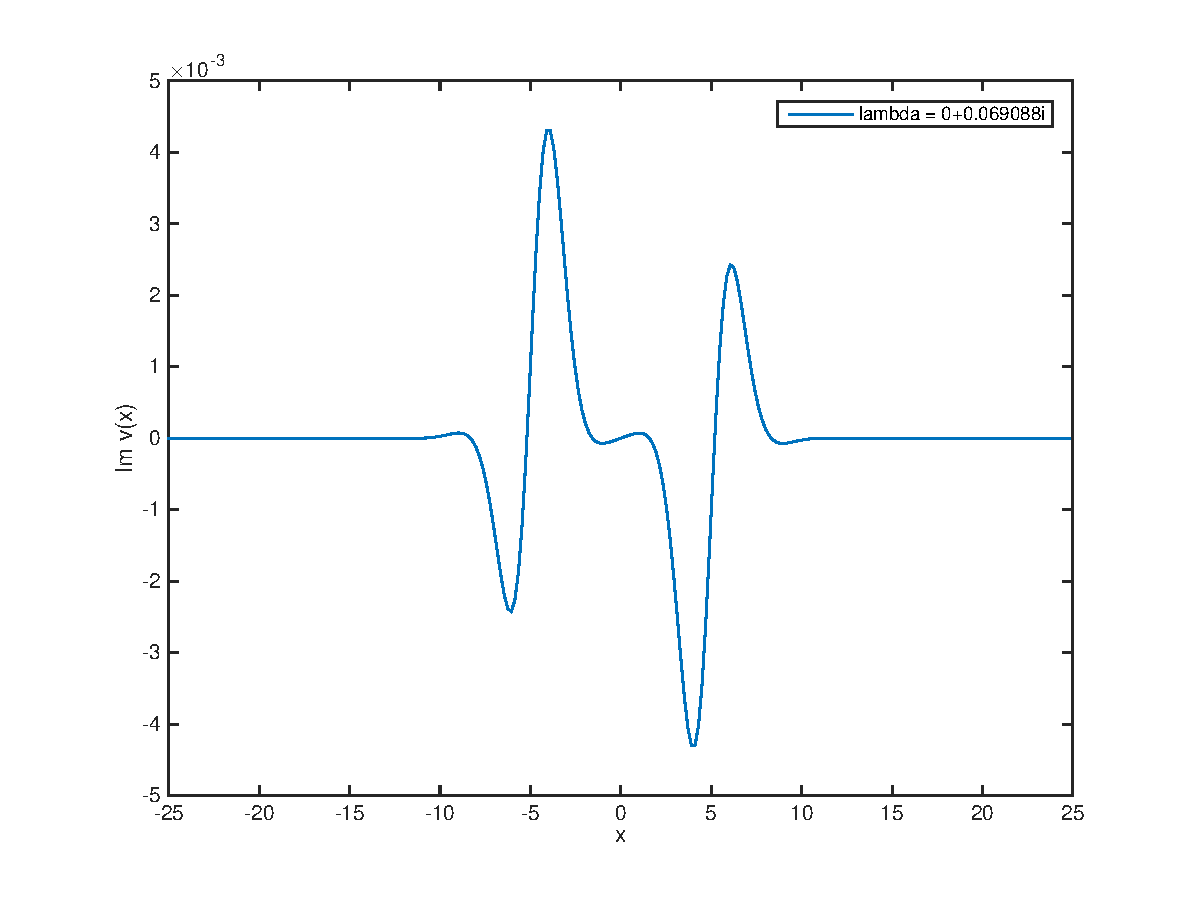
\includegraphics[width=8.5cm]{four10dp2eigenfnsimag_after}
	\caption{Real and imaginary parts of eigenfunctions corresponding to eigenvalue with positive imaginary part for linearization about double pulse 2(4) after rotation by unit complex number and elimination of small real part of eigenvalue using \texttt{fsolve}. Wave speed $c = 10$, Fourier spectral methods, $N = 256$}
\end{figure}

\begin{figure}[H]
	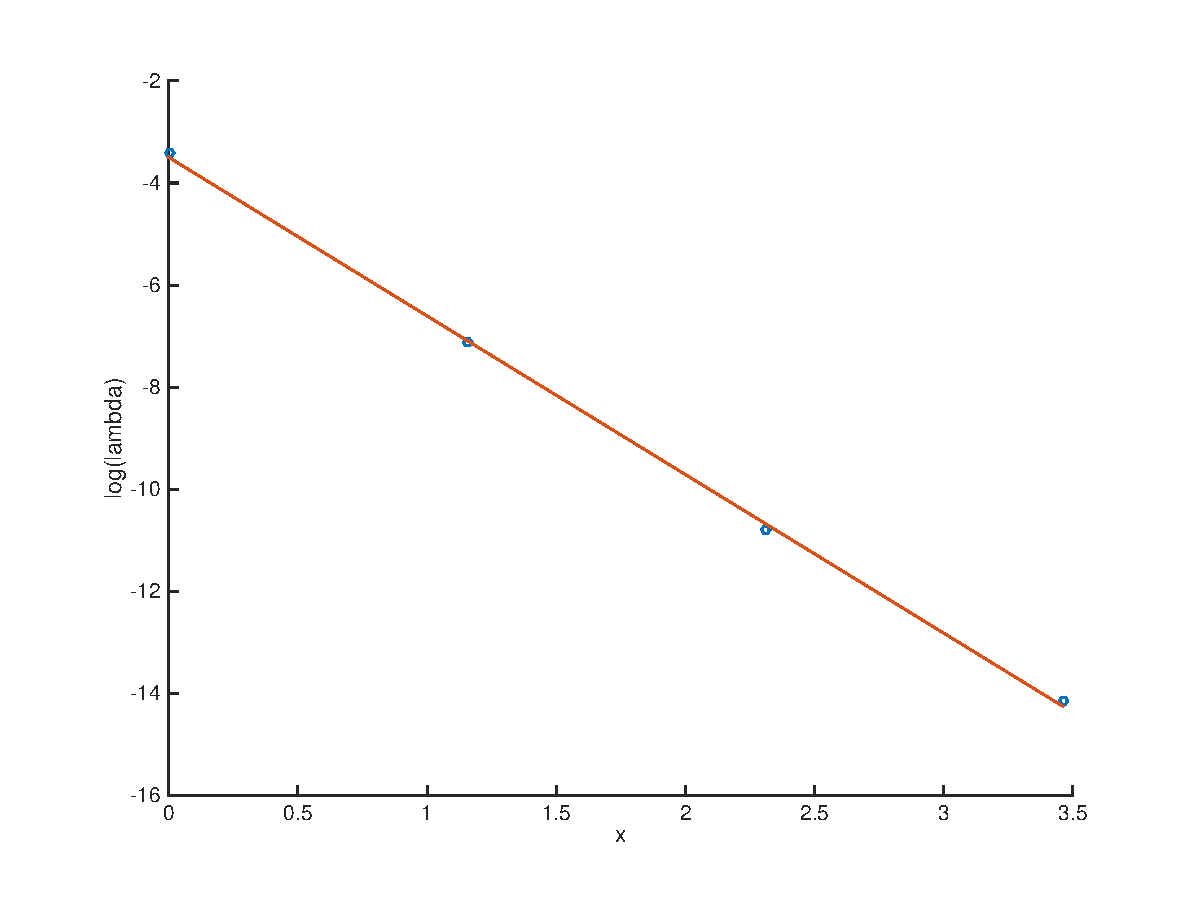
\includegraphics[width=8.5cm]{decayinteigenvalue}
	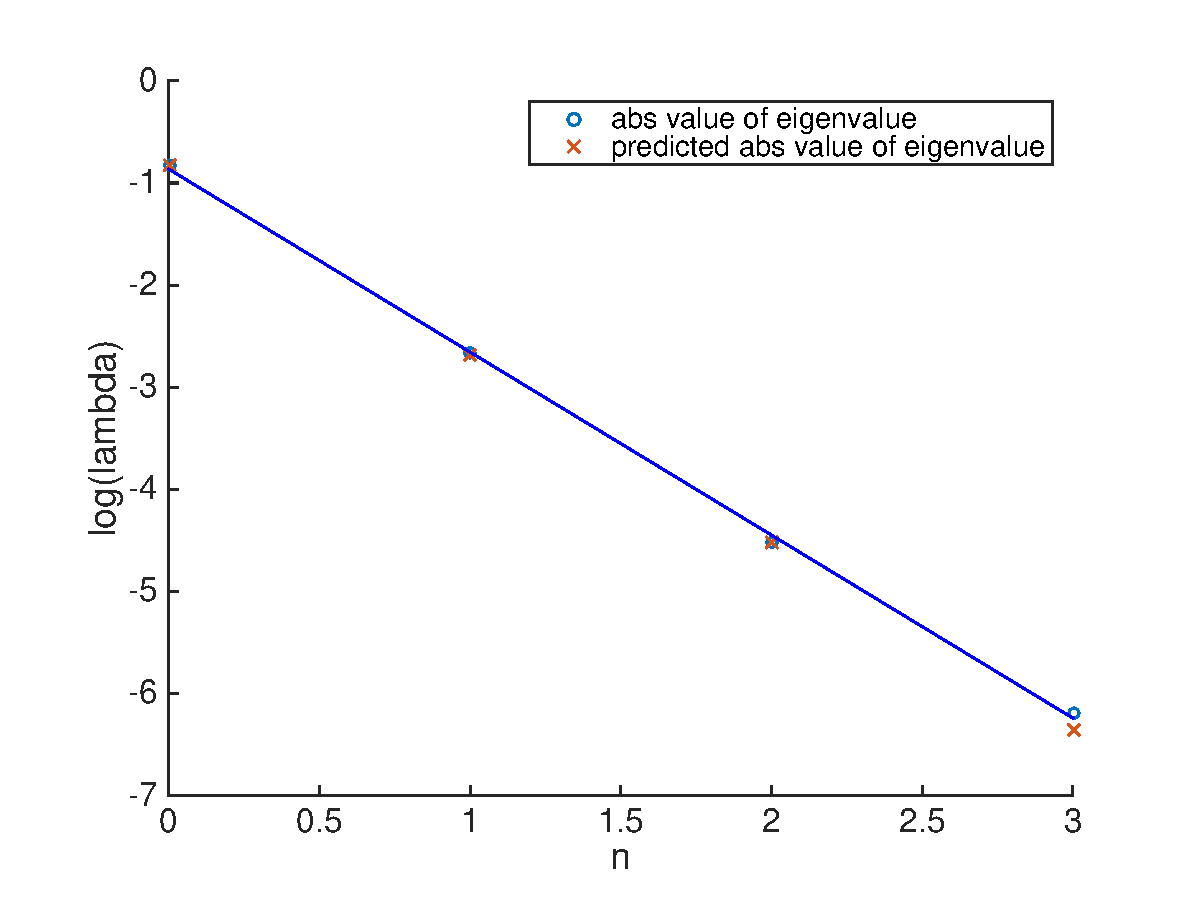
\includegraphics[width=8.5cm]{decayeigenvalue}
	\caption{Exponential decay of eigenvalues of linearized integrated (4th order) operator (left) and absolute value of eigenvalues of linearized KdV (5th order) operator (right). Waves are 2(2), 2(3), 2(4), and 2(5). Wave speed $c = 10$, Fourier spectral methods, $N = 256$}
\end{figure}

\begin{figure}[H]
\begin{tabular}{l|lll}
 Double Pulse   & $c = 10$            & $c=7.5$                        & $c=5$        \\ \hline
  2(2) &     $\pm 0.4352$             & $\pm 0.2730$                   & $\pm 0.1363$ \\ 
  2(3) &     3.5702e-08 $\pm 0.0691i$ & 1.2186e-08 $\pm 0.0413i$       & 2.0229e-09 $\pm 0.0190i$\\ 
  2(4) &     $\pm 0.0109$             & $\pm 0.0064$                   & \\ 
  2(5) &    -2.4222e-12 $\pm 0.0020i$ & 8.0169e-13 $\pm$ 9.4458e-04$i$ & \\
\end{tabular}
\caption{Eigenvalues for linearization about double pulses 2(2), 2(3), 2(4), and 2(5) for wave speeds $c = 10, 7.5, 5$. Chebyshev spectral methods, $N = 257$}
\end{figure}

\begin{figure}[H]
\begin{tabular}{l|ll}
 Double Pulse   & $\max{|Jv - \lambda v|}$ before \texttt{fsolve} & $\max{|Jv - \lambda v|}$ after \texttt{fsolve}\\ \hline
  2(3) & 3.0291e-06 & 8.5938e-09 \\
  2(5) & 1.1501e-06 & 1.2419e-10 \\
\end{tabular}
\caption{Maximum of eigenvalue problem $|Jv - \lambda v|$ before and after using Matlab's \texttt{fsolve} to eliminate small real part of eigenvalue. Wave speed $c = 10$, Chebyshev spectral methods, $N = 257$.}
\end{figure}

\subsection{Time stepping}

\begin{figure}[H]
	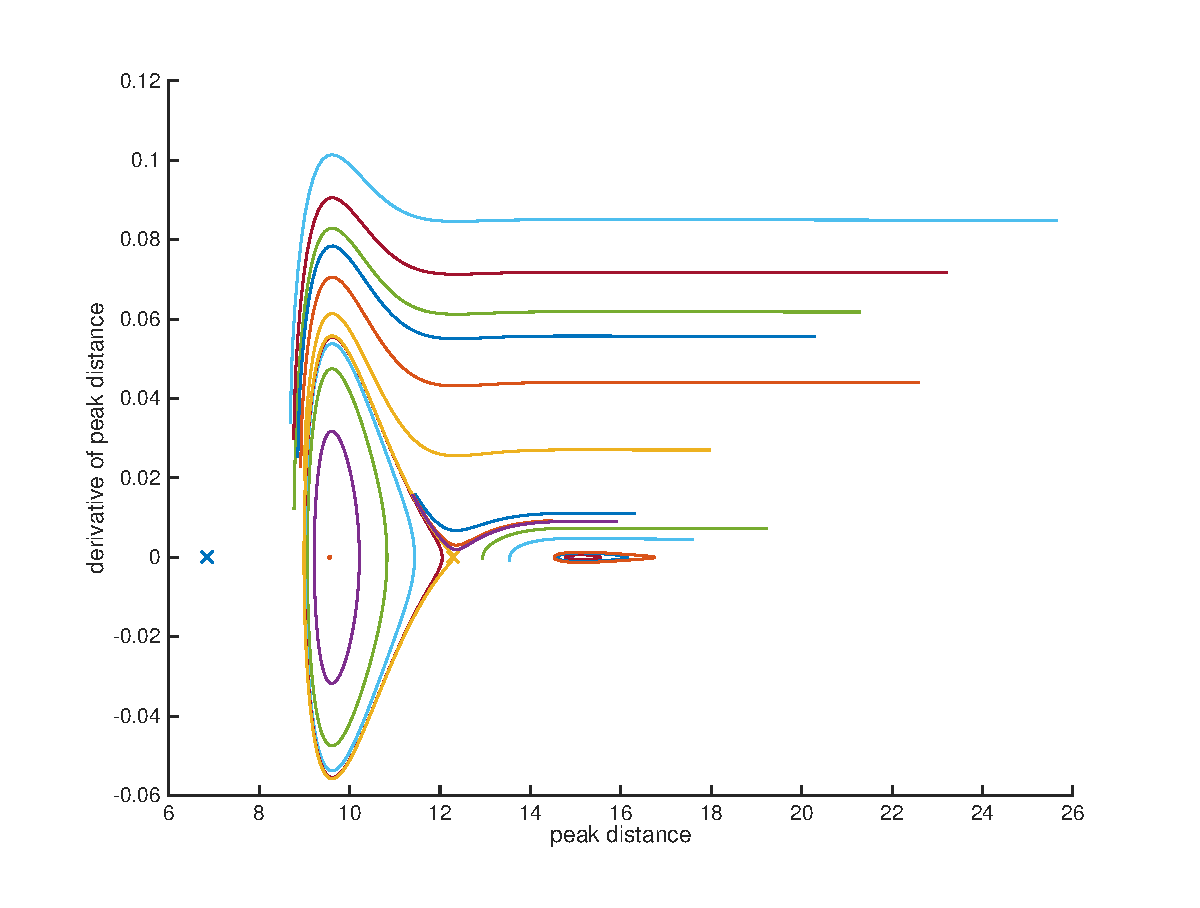
\includegraphics[width=8.5cm]{phaseportrait1}
	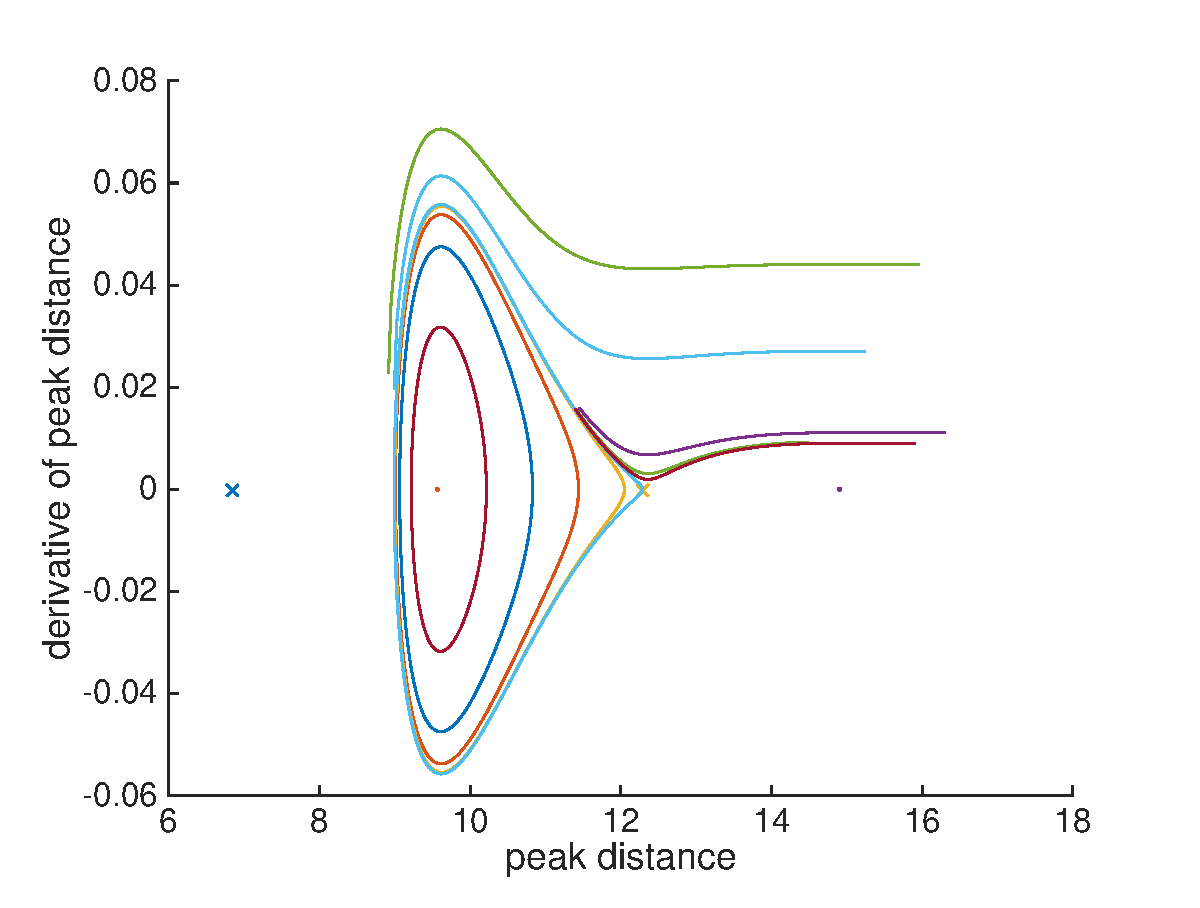
\includegraphics[width=8.5cm]{phaseportrait2}
	\caption{Phase portait for reduced two-dimensional system. Variables are distance between two pulses and its derivative. Wave speed $c = 10$, Chebyshev spectral methods, $N = 256$}
\end{figure}

\subsection{Multipulses}
\begin{figure}[H]
	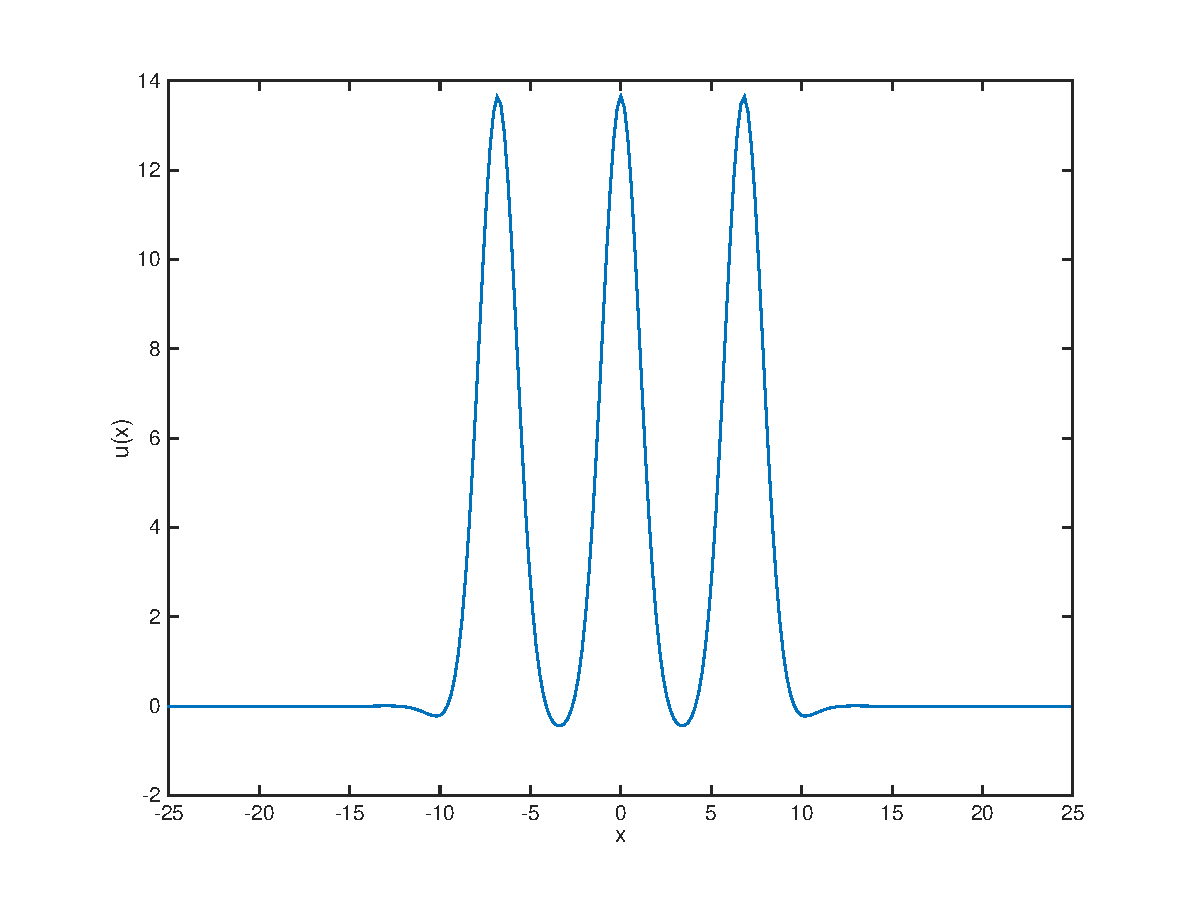
\includegraphics[width=8.5cm]{four10um1_3}
	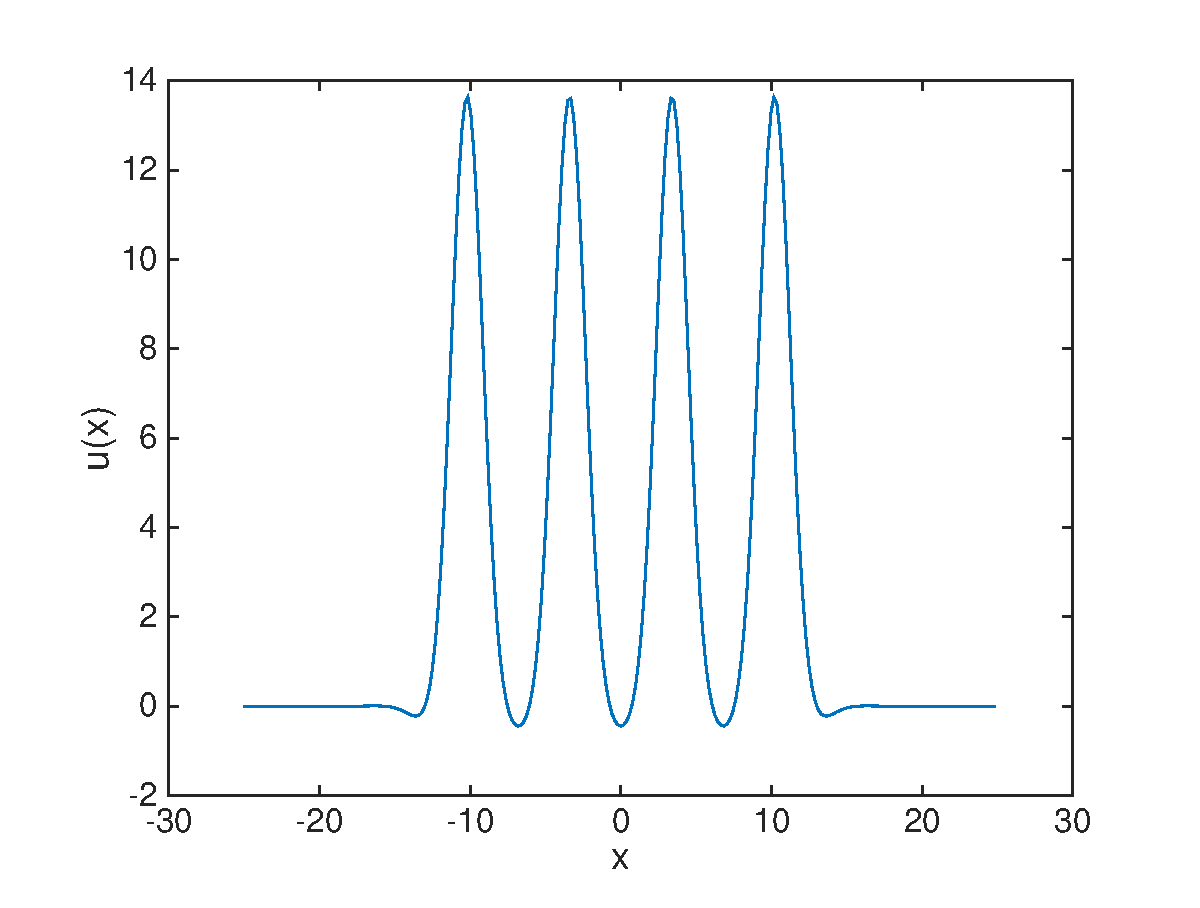
\includegraphics[width=8.5cm]{four10um1_4.eps}
	\caption{Multipulses 3(2,2) and 4(2,2,2). Wave speed $c = 10$, Fourier spectral methods, $N = 256$. }
\end{figure}

\begin{figure}[H]
	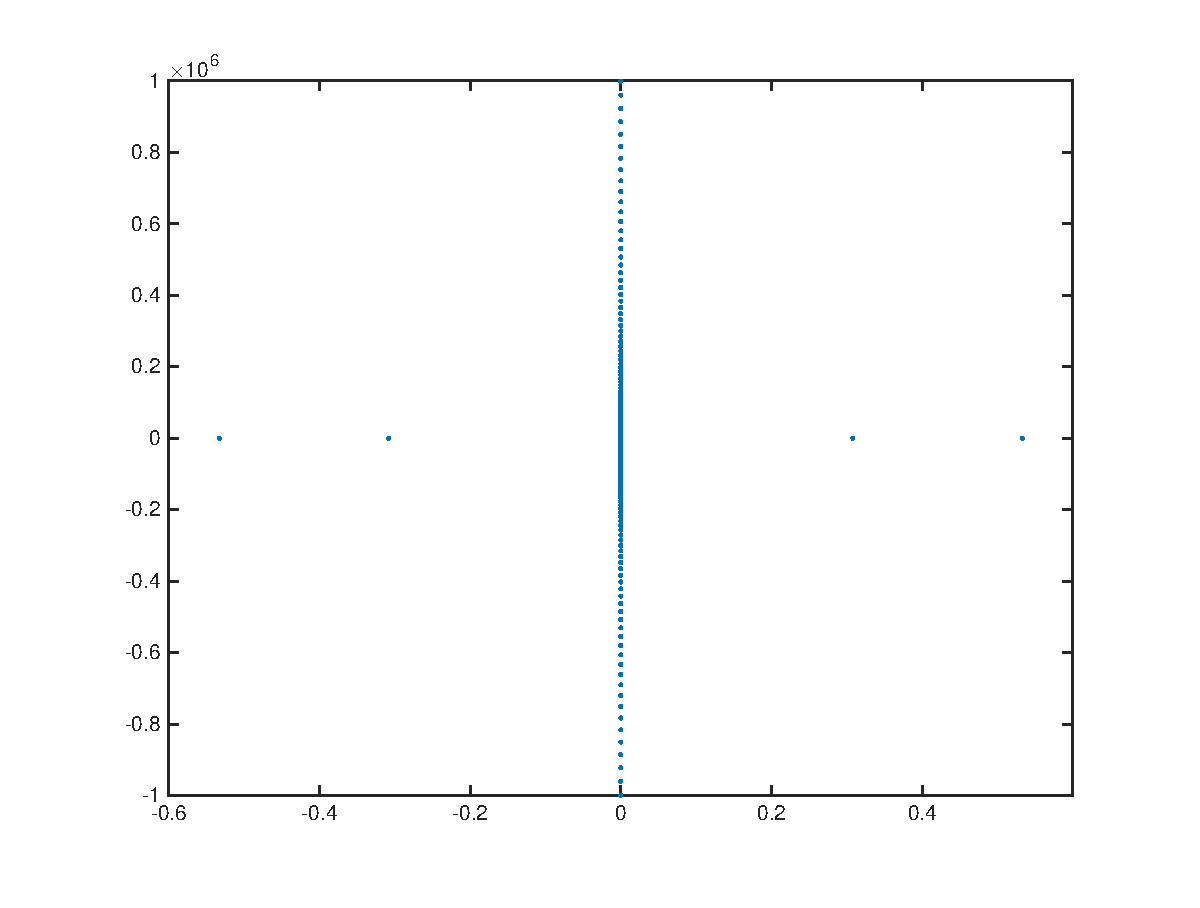
\includegraphics[width=8.5cm]{four10um1_3lambda}
	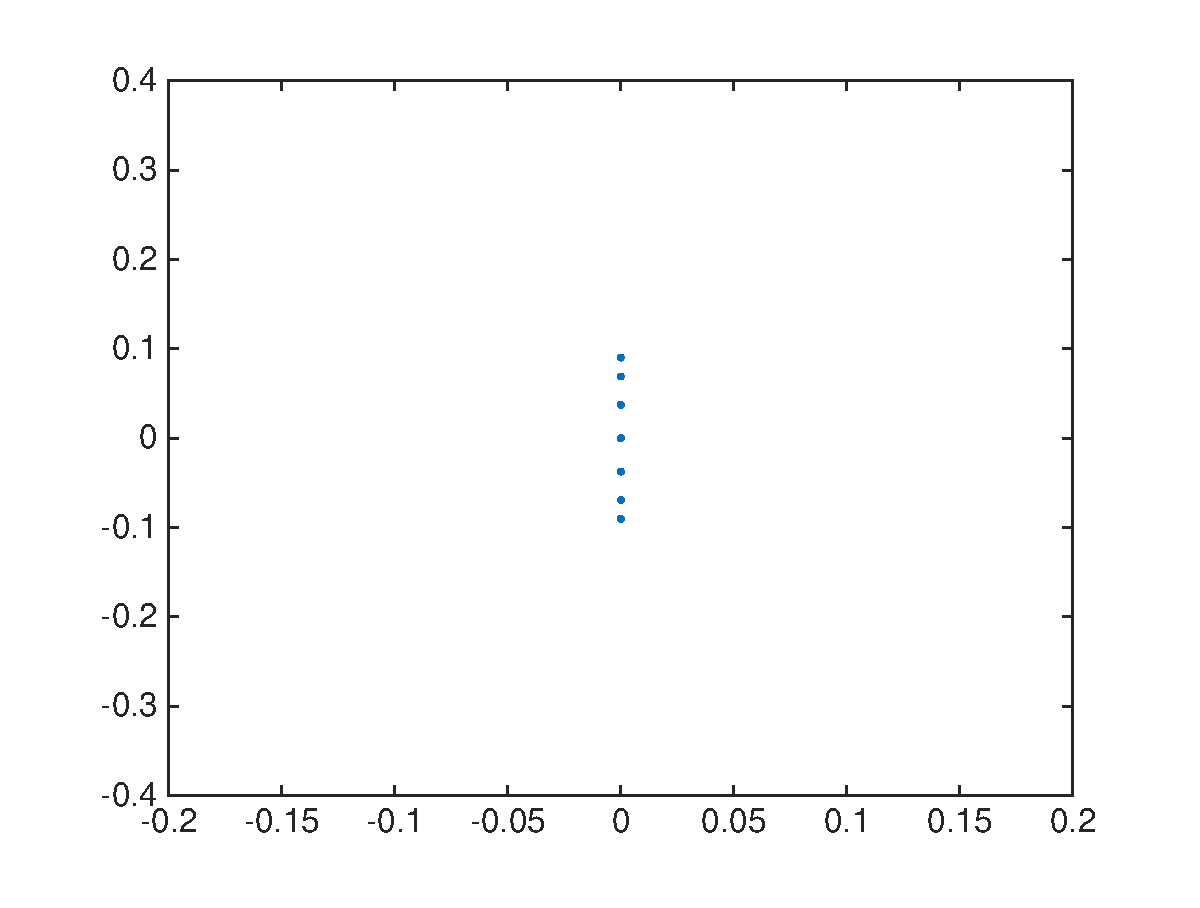
\includegraphics[width=8.5cm]{four10um1_4lambda}
	\caption{Eigenvalues of 5th order KdV for multipulses 3(2,2) and 4(2,2,2). Wave speed $c = 10$, Fourier spectral methods, $N = 256$. }
\end{figure}

\begin{figure}[H]
\begin{tabular}{l|l}
  Pulse    &  Nonzero Eigenvalues \\ \hline
  2(2)     &     $\pm 0.4352$  \\ 
  3(2,2)   &     $\pm 0.5328, \pm 0.3079$   \\ 
  4(2,2,2) &     $\pm 0.5683, \pm 0.4353, \pm 0.2358 $  \\ 
\end{tabular}
\caption{Eigenvalues of 5th order KdV for multipulses 3(2,2) and 4(2,2,2). Wave speed $c = 10$, Fourier spectral methods, $N = 256$. }
\end{figure}

\begin{figure}[H]
	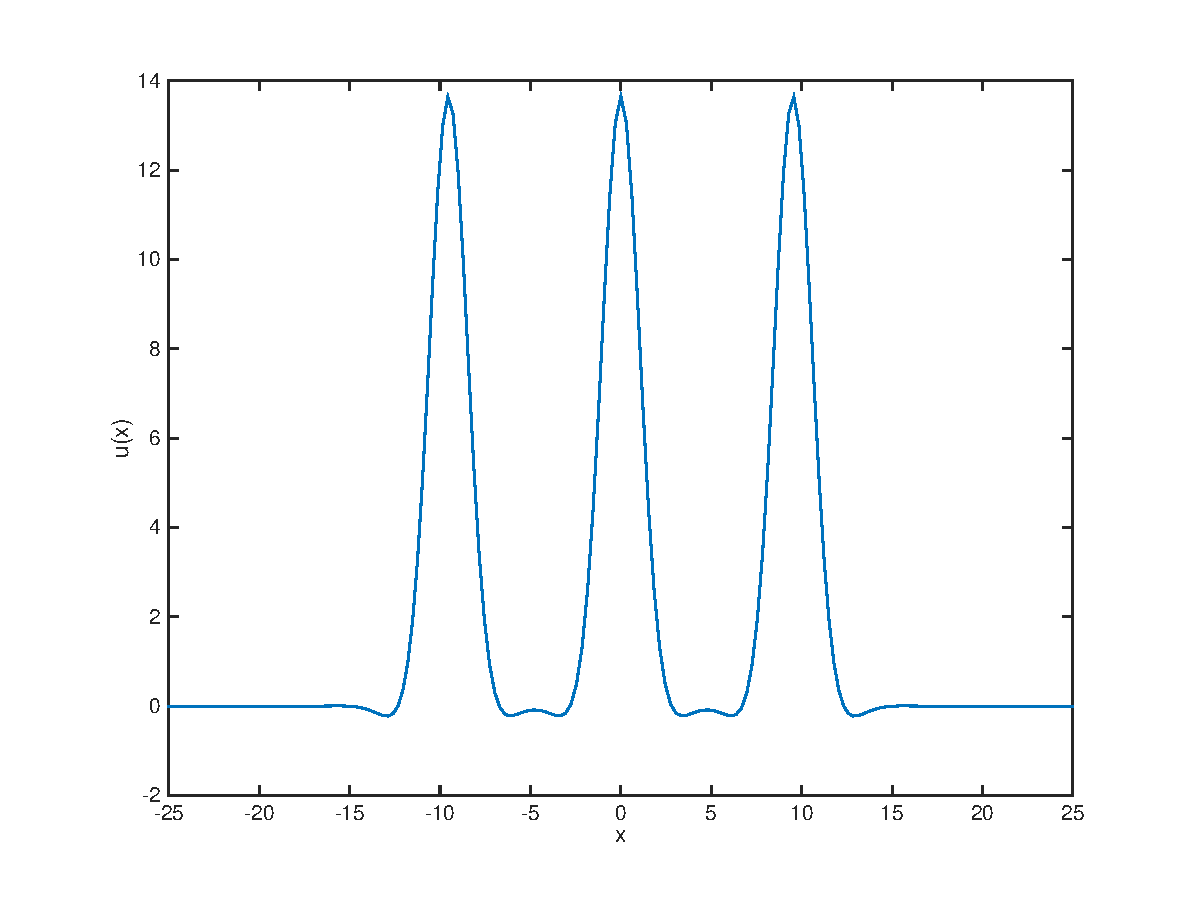
\includegraphics[width=8.5cm]{cheb10um2_3.eps}
	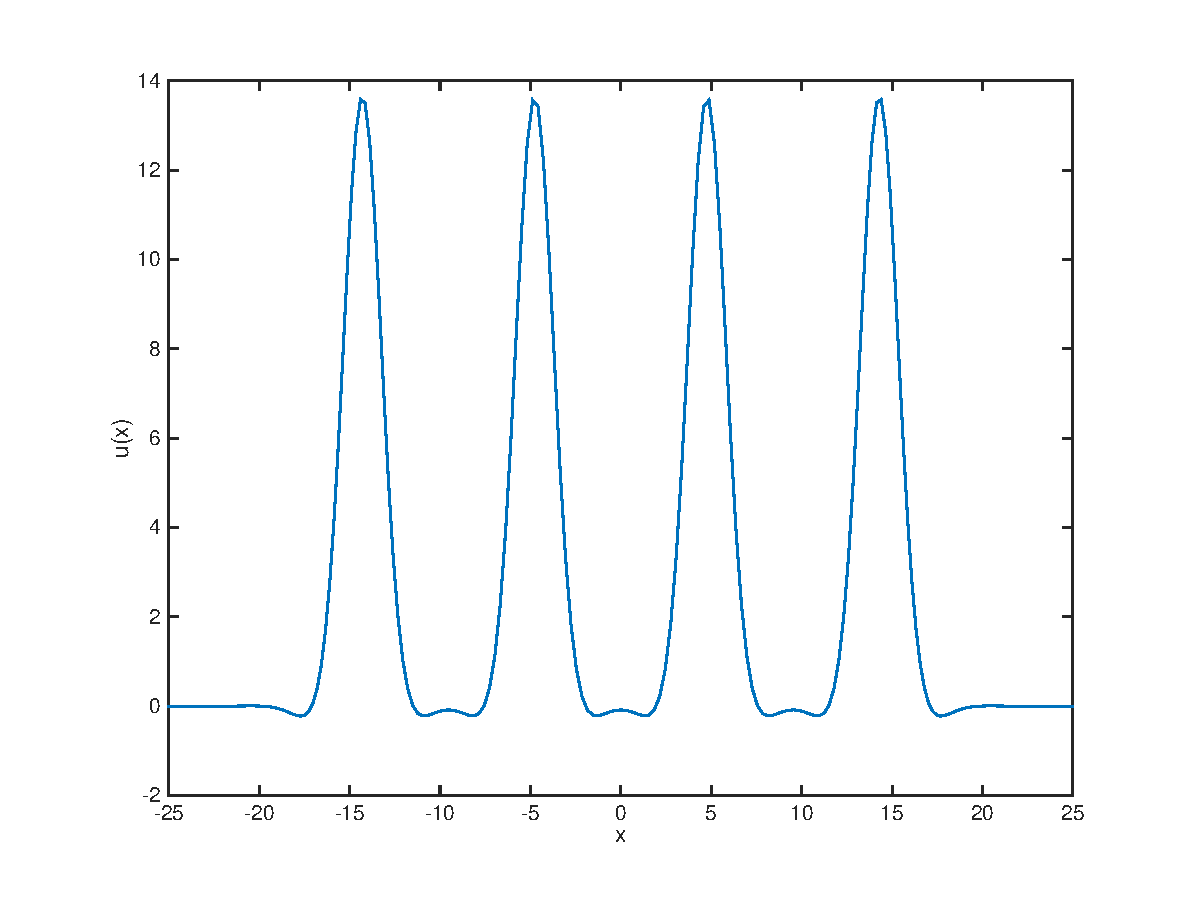
\includegraphics[width=8.5cm]{cheb10um2_4.eps}
	\caption{Multipulses 3(3,3) and 4(3,3,3). Wave speed $c = 10$, Chebyshev spectral methods, $N = 257$.}
\end{figure}

\begin{figure}[H]
	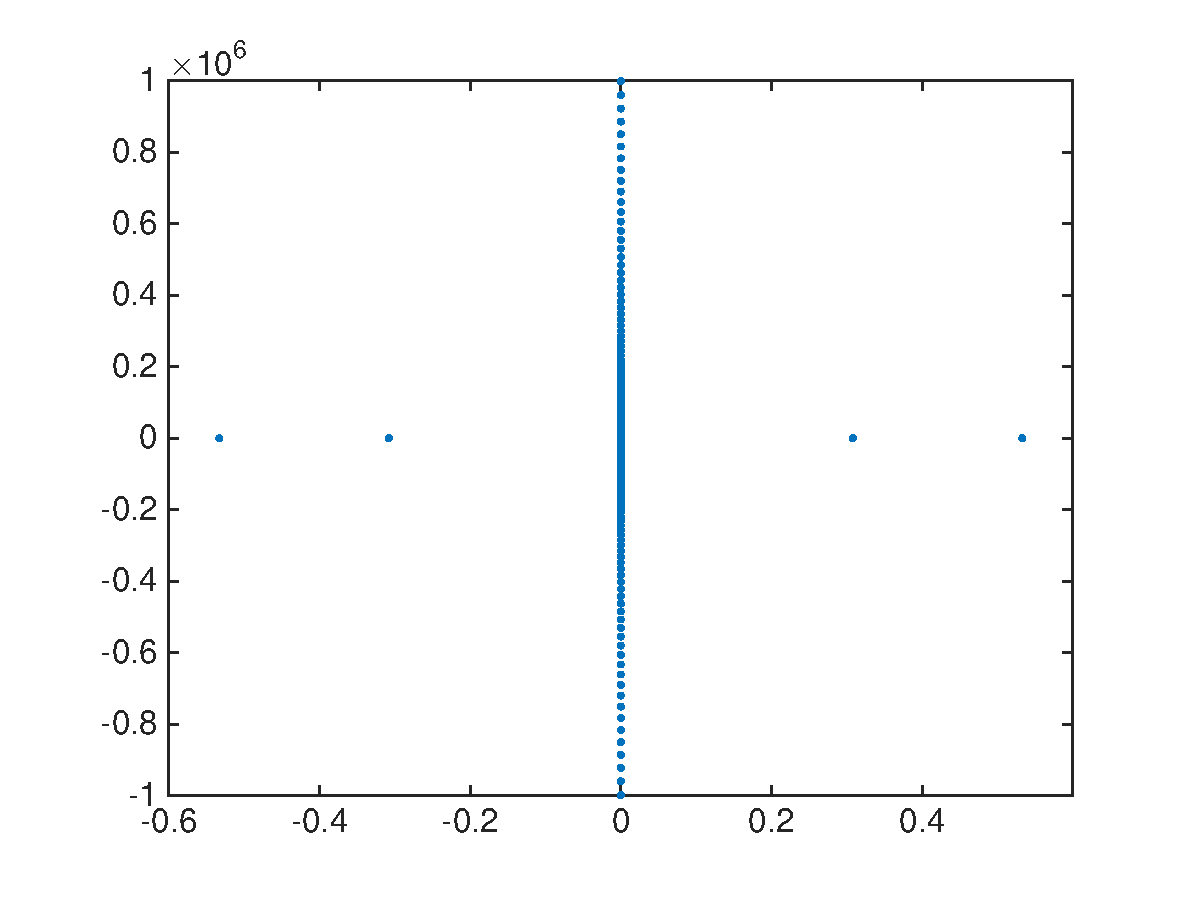
\includegraphics[width=8.5cm]{cheb10um2_3lambda.eps}
	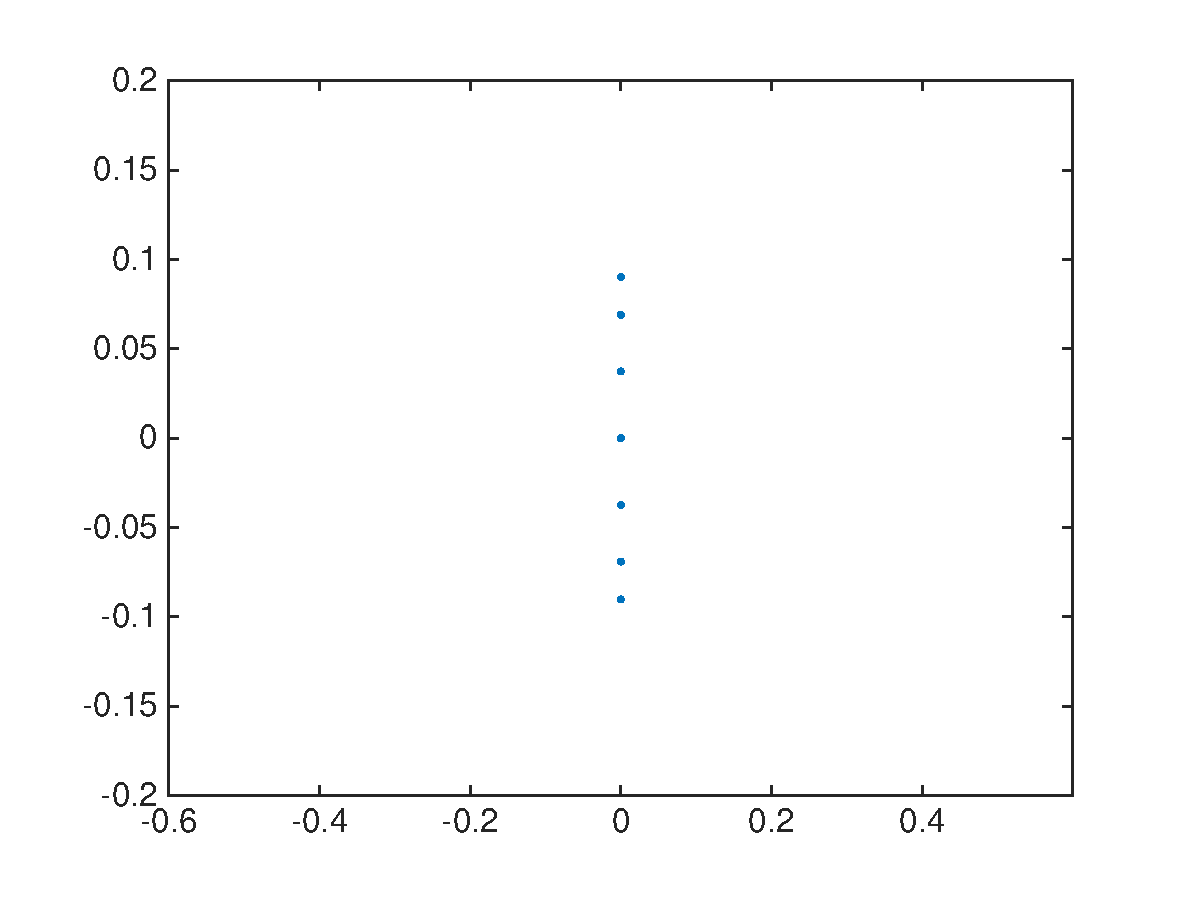
\includegraphics[width=8.5cm]{cheb10um2_4lambda.eps}
	\caption{Eigenvalues near origin of 5th order KdV for multipulses 3(3,3) and 4(3,3,3). Wave speed $c = 10$, Fourier spectral methods, $N = 256$. }
\end{figure}

\begin{figure}[H]
\begin{tabular}{l|l}
  Pulse    &  Nonzero Eigenvalues \\ \hline
  2(3)     &     $\pm 0.0691i$ \\ 
  3(3,3)   &     $\pm 0.0846i$, $\pm 0.0489i$   \\ 
  4(3,3,3) &     $\pm 0.0903i$, $\pm 0.0691i$, $\pm 0.0374i$ \\ 
\end{tabular}
\caption{Eigenvalues of 5th order KdV for multipulses 3(3,3) and 4(3,3,3). Tiny real part of eigenvalues found by \texttt{eig} has been removed using \texttt{fsolve}, with improvement in $\max{|Jv - \lambda v|}$. Wave speed $c = 10$, Fourier spectral methods, $N = 256$. }
\end{figure}

\section{References}

\end{document}